\documentclass[10pt,a4paper]{article}

\usepackage[utf8]{inputenc}
\usepackage{graphicx}

\usepackage[margin=19mm]{geometry}
\parskip 6.4pt

\usepackage{amsmath}
\usepackage{mathtools}
\usepackage{esint}
\usepackage{amssymb}
\usepackage{amsfonts}
\usepackage{multicol}
\usepackage{tabularx}
\usepackage{booktabs}
\usepackage{url}
\usepackage[colorlinks=true, linkcolor=black, urlcolor=black, citecolor=black]{hyperref} 

\usepackage{subfiles}

\usepackage{listings}
\usepackage{xcolor}

%%%%%%%%%%%%%%%%%%%%%%%%%%%%%%%%%%%%%%%%%%%%%%%%%%%%%%%%%%%%

% --- GitHub-Inspired Colors ---
\definecolor{github-bg}{HTML}{F6F8FA}      
\definecolor{github-border}{HTML}{E1E4E8}  

\lstdefinestyle{github-bash}{
  backgroundcolor=\color{github-bg},
  rulecolor=\color{github-border},
  frame=single,
  basicstyle=\ttfamily\small,
  showstringspaces=false,
  numbers=left,
  numberstyle=\tiny\color{gray},
  stepnumber=1,
  numbersep=10pt,
  tabsize=2,
  breaklines=true,
  breakatwhitespace=true,
  captionpos=b,
  xleftmargin=0.05\textwidth,
  xrightmargin=0.05\textwidth,
}

\lstset{style=github-bash}

%%%%%%%%%%%%%%%%%%%%%%%%%%%%%%%%%%%%%%%%%%%%%%%%%%%%%%%%%%%%

\title{Relazione Progetto Boids}
\author{Francesco Bartoli}
\date{}

\begin{document}

\maketitle

\hypertarget{toc}{}
\tableofcontents

\setlength{\parindent}{0pt}

\section*{Cambiamenti}

Di seguito sono elencati i cambiamenti all'interno del progetto intercorsi dall'ultima consegna.

\begin{itemize}
    \item La classe boid è ora una \texttt{struct}, in quanto non era presente nessun invariante di classe.
    \item I file di generazione di numeri casuali hanno avuto dei cambiamenti. In particolare, ora vi è solo l'header, e l'engine, non è più una variabile globale, ma è passato come parametro ad ogni singola funzione che ne facesse utilizzo.
    \item Le funzioni di \texttt{statistics.hpp} sono state rivisitate in modo da produrre un codice molto più performante. Ora non vengono più utilizzati grandi vettori inutilmente per il calcolo delle statistiche degli stormi.
\end{itemize}

Anche la relazione è stata modificata in modo da rispecchiare i cambiamenti apportati, sia nella descrizione dei file che compongono il progetto, sia nelle istruzioni alla compilazione e all'installazione, ad esempio.

\newpage

\parskip 1.6pt
\section{Introduzione}
\subsection{Scopo}
Il programma ha come obiettivo quello di simulare in uno spazio bidimensionale il comportamento di stormi di uccelli in volo, che verranno indicati con il nome di \textit{boids}.

\subsection{Installazione}

Le istruzioni su come compilare, testare, eseguire sono presentate nel README.md del progetto, riportato qui sotto:

Build instructions are for \textbf{Ubuntu 22.04}.

\subsubsection{Prerequisites}

\href{https://github.com/SFML/SFML}{SFML} (2.6): Library for graphic representation. \\
\href{https://github.com/texus/TGUI}{TGUI} (1.0): Library for graphic interface.

\subsubsection{SFML and TGUI Installation}

Install SFML:

\begin{lstlisting}[style=github-bash]
sudo apt install libsfml-dev
\end{lstlisting}

Install TGUI:

\begin{lstlisting}[style=github-bash]
sudo add-apt-repository ppa:texus/tgui
sudo apt update
sudo apt install libtgui-1.0-dev
\end{lstlisting}

\subsubsection{Clone the Repository}

\begin{lstlisting}[style=github-bash]
git clone --depth=1 https://github.com/Evyal/boids.git
cd boids
\end{lstlisting}

\subsubsection{Build the Project}

\begin{itemize}
    \item \title{\textbf{Create the build directory}}

          \begin{lstlisting}[style=github-bash]
mkdir build
\end{lstlisting}

    \item \title{\textbf{Configure CMake with Ninja Multi-Config:}}

          \begin{lstlisting}[style=github-bash]
cmake -S . -B build -G "Ninja Multi-Config"
\end{lstlisting}

    \item \title{\textbf{Build the project}}

    Debug Mode:
          \begin{lstlisting}[style=github-bash]
cmake --build build --config Debug
\end{lstlisting}

Release Mode:
          \begin{lstlisting}[style=github-bash]
cmake --build build --config Release
\end{lstlisting}    
\end{itemize}


\subsubsection{Running the program}

    Debug Mode:
          \begin{lstlisting}[style=github-bash]
cd build/Debug
./boids
\end{lstlisting}

Release Mode:
          \begin{lstlisting}[style=github-bash]
cd build/Release
./boids
\end{lstlisting}    



\newpage

\parskip 6.4pt

\section{Struttura del programma}

I file del progetto sono organizzati in sottocartelle, nello specifico i \texttt{.cpp} si trovano nella \texttt{/source}, mentre i rispettivi header sono situati nella \texttt{/include}. La directory \texttt{/testing} contiene i file di testing, e infine in \texttt{/assets} è presente il font utilizzato nell'interfaccia grafica.

\subsection{Regole di volo}

I \textit{boids} seguono delle regole di volo, che ne determinano il comportamento. Ad ogni istante, il programma modifica le velocità e le posizioni dei \textit{boids} attraverso le seguenti formule:

\begin{equation*}
    \vec{v}_{bi} = \vec{v}_{bi} + \vec{v}_S + \vec{v}_A + \vec{v}_C + \vec{v}_R
\end{equation*}

\begin{equation*}
    \vec{x}_{bi} = \vec{x}_{bi} + \vec{v}_{bi} \cdot k
\end{equation*}

Dove $k$ è un fattore di scala, mentre $\vec{v}_S$, $\vec{v}_A$, $\vec{v}_C$, e $\vec{v}_R$ sono rispettivamente:

\vspace{2mm}

\textbf{Separazione}
\begin{equation*}
    \vec{v}_S = -s \sum_{j \neq i} (\vec{x}_{b_j} - \vec{x}_{b_i}) \quad \text{se} \quad \left| \vec{x}_{b_i} - \vec{x}_{b_j} \right| < d_s
\end{equation*}

\vspace{2mm}

\textbf{Allineamento}

\begin{equation*}
    \vec{v}_A = a \left[ \frac{1}{n} \sum_{j \neq i} (\vec{v}_{b_j} - \vec{v}_{b_i}) \right] \quad \text{se} \quad \left| \vec{x}_{b_i} - \vec{x}_{b_j} \right| < i
\end{equation*}

\vspace{2mm}

\textbf{Coesione}

\begin{equation*}
    \vec{x_{c_i}} = \frac{1}{n} \sum_{j \neq i} \vec{x}_{b_j} \quad \text{se} \quad \left| \vec{x}_{b_i} - \vec{x}_{b_j} \right| < i
\end{equation*}

\vspace{2mm}

\begin{equation*}
    \vec{v}_C = c (\vec{x}_{c_i} - \vec{x}_{b_j})
\end{equation*}

Dove $n$ è numero di \textit{boids} dello stormo nel range di interazione di ciascun \textit{boid}, e non è un valore fisso.

E $s, ds, a, c, i$ sono parametri della simulazione, e nel progetto sono indicati con i nomi di \textit{separationStrength}, \textit{separationRange}, \textit{alignmentStrength}, \textit{cohesionStrength} e \textit{interactionRange}.

\vspace{2mm}

\textbf{Repulsione}

La formulazione matematica di questa regola è analoga a quella della separazione e determina l'allontanamento tra \textit{boids} di stormi differenti introducendo due nuovi parametri $r, dr$, che nel progetto sono indicati con i nomi di \textit{repelStrength} e \textit{repelRange}.

\vspace{2mm}

\textbf{Interazione \textit{On Click}}

\begin{equation*}
    \vec{v} = \pm p \sum_{j} (\vec{x}_{b_j} - \vec{x}) \quad \text{se} \quad \left| \vec{x}_{b_j} - \vec{x} \right| < i
\end{equation*}

Anche questa regola ha una formula analoga a quella della separazione e permette all'utente di interagire con i \textit{boids}. Il $\pm$ è dovuto al fatto che questa interazione può essere sia attrattiva che repulsiva mentre $\vec{x}$ è il punto in cui l'utente ha cliccato. Il parametro che determina l'intensità di questa interazione prende il nome di \textit{clickStrength} all'interno del progetto.

\newpage

\subsection{Files}

Tutti i file del progetto sono stati inseriti nel namespace \texttt{ev}.

\subsubsection{\texttt{constants.hpp}}

Header file che definisce i valori delle costanti usate nel progetto raggruppandole nel namespace \texttt{constants}. Alcuni esempi sono limiti di posizione o velocità per i \textit{boids}, parametri di interazione di default, o ulteriori valori fissi per l'inizializzazione degli elementi dell'interfaccia grafica. Uno dei principali vantaggi di questo approccio è la possibilità di cambiare valori riutilizzati in diverse unità del programma, tutti da un unico punto, conferendo una maggiore facilità della loro modifica.

\subsubsection{\texttt{structs.hpp}}

Header contenente la definizione di alcune \texttt{struct} designate prevalentemente ad impacchettare dei valori usati per inizializzare bottoni o altri elementi di interfaccia grafica. Trovano particolare utilità come parametri delle funzioni che inizializzano tali elementi, aiutando a mantenere il codice più pulito. Un esempio è la \textit{struct} \texttt{TguiPar} che contiene i parametri per inizializzare un generico elemento di interfaccia grafica, da cui seguono alcune struct derivate, come \texttt{SlidersPar}. È presente un'unica struct che non ha a che fare con la parte grafica, e contiene le variabili che parametrizzano l'interazione dei \textit{boids} negli stormi.

\subsubsection{\texttt{boid.hpp/cpp}}

File che si occupa dell'implementazione della struct \texttt{Boid} e di tutte le funzioni ausiliari necessarie per gestirne il comportamento. Le variabili utilizzate all'interno dell'aggregato per descrive il comportamento dei \textit{boids} sono posizione e velocita, sotto forma di \texttt{sf::Vector2f} forniti da SFML. Inoltre sono presenti le funzioni che lavorano su elementi della classe, come per esempio \texttt{distance} che calcola la distanza fra \textit{boids} o \texttt{minimumSpeedControl()} che ha il compito di assicurarsi che il \textit{boid} in questione abbia una velocità compresa all'interno dei limiti prestabiliti, ed eventualmente modificarla. È importante sottolineare che la velocità limite non è stata intesa all'interno del progetto come un'invariante di classe, ma semplicemente un limite imposto durante la simulazione per assicurarsi un comportamento ordinato, infatti non è vietato che un \textit{boid} possieda una velocità superiore al limite prestabilito, in quanto questo non invalida nessuna delle funzioni che lo utilizzano.

\subsubsection{\texttt{flock.hpp/cpp}}

File di implementazione della classe \texttt{Flock} che determina la struttura collettiva dei \textit{boids} all'interno di uno stormo. La classe presenta numerose variabili statiche, condivise da tutti gli stormi, che costituiscono i parametri dell'interazione tra \textit{boids}, e due variabili membro private, la prima un vettore di \textit{boids}, in cui sono contenuti i \textit{boid} che compongono lo stormo, e l'altra che determina il colore dello stormo. Il vettore di \textit{boids} deve contenere almeno due elementi, e il modo in cui si è scelto di gestire un tentativo di inizializzare un'istanza appartenente alla classe \texttt{Flock} con meno di due elementi, è attraverso il lancio di un eccezione. In fase di debug, per assicurarsi che la classe non permettesse l'utilizzo dei suoi metodi su stormi con meno di due \textit{boids}, sono stati inseriti multipli \texttt{assert()} all'interno del corpo di quest'ultimi. La parte restante della classe è designata all'implementazione delle regole che determinano il comportamento degli stormi, e della funzione \texttt{updateFlock()} che si occupa di aggiornare lo stato dello stormo. Quest'ultima funzione ne ha una \texttt{overloaded}, in grado di prendere come argomento le velocità da sommare dovute alla repulsione con altri stormi.

\subsubsection{\texttt{random.hpp}}

Header che si occupa della generazione di numeri casuali. Sono presenti una funzioni base per generare numeri casuali di tipo \texttt{size\_t} o \texttt{float}, e funzioni più complesse per generare posizioni e velocità dei \textit{boids} in range prestabiliti.

\subsubsection{\texttt{statistics.hpp/cpp}}

File che si occupa del calcolo delle statistiche restituite a schermo, riguardanti valori medi e deviazioni standard delle posizioni e velocità dei \textit{boids}. Ad esempio, la funzione \texttt{calculateDistances()} calcola la distanza media tra boids e la sua deviazione standard, mentre \texttt{calculateToroidalDistances()} fa lo stesso ma in geometria toroidale.

\subsubsection{\texttt{graphics.hpp/cpp}}

Breve file che contiene due funzioni. La prima si occupa di creare la figura geometrica che rappresenta graficamente i \textit{boids}, posizionata ed orientata correttamente. La seconda costruisce un rettangolo (\texttt{sf::Rectangle}) prendendo come parametro una delle struct definite nel file sopracitato, con lo scopo di migliorare la leggibilità del codice nella creazione dell'interfaccia.

\subsubsection{\texttt{switchbutton.hpp/cpp}}

La classe \texttt{SwitchButton} introduce la funzionalità di un bottone che può trovarsi in due stati, non fornita da TGUI, e si è cercato di seguire le convenzioni di TGUI nella creazione delle funzioni membro. In particolare è presente un costruttore, che crea un oggetto della classe, ed una funzione \texttt{create()} che restituisce uno \texttt{std::shared\_ptr} che punta all'oggetto.

\subsubsection{\texttt{gui.hpp/cpp}}

In quest'ultimo file è definita la classe che contiene gli elementi necessari a realizzare l'interfaccia grafica del programma, e si occupa di coordinare gli altri file all'interno di essa. La classe contiene diversi membri privati, come ad esempio la \texttt{sf::RenderWindow}, per la raffigurazione grafica, l'elemento \texttt{tgui::Gui} per il funzionamento dei pulsanti, un vettore che contiene gli stormi attivi, e così via. Le funzioni al suo interno sono prevalentemente di \textit{setup}, e sono organizzate in tre macro-aree, ciascuna con lo scopo di configurare la propria opzione di menù. Infine sono presenti ulteriori funzioni, come quella di creazione del menù (\texttt{createThreeWaySwitch()}), e quelle di gestione, creazione e distruzione degli stormi.

In ultima analisi, la classe \texttt{Gui} è responsabile del generale funzionamento del programma. Nel main è sufficiente costruire un elemento della classe, utilizzare il metodo \texttt{setup()} che lo configura correttamente e infine chiamare il metodo \texttt{run()} che contiene le istruzioni da seguire durante l'esecuzione.

\newpage

\section{Interfaccia della simulazione}
%descrizione del formato di input e di output, possibilmente con degli esempi

Anche questa parte derivante parzialmente dal README.md del progetto.

% \begin{center}
%     \includegraphics[width=1.0\textwidth]{images/interface.png}
% \end{center}

% \maketitle{\textbf{Features}}

% - Random generation of flocks at the beginning of the simulation \\
% - Different modes for behaviour at borders \\
% - Statistics display for each active flock \\
% - Interactive controls for adding or removing flocks \\
% - Adjustable parameters for interactions between \textit{boids} \\

% \begin{center}
%     \includegraphics[width=0.32\textwidth]{images/option1.png}
%     \includegraphics[width=0.32\textwidth]{images/option2.png}
%     \includegraphics[width=0.32\textwidth]{images/option3.png}
% \end{center}

\begin{center}
    \includegraphics[width=1.0\textwidth]{../images/interface.png}
\end{center}

\maketitle{\textbf{Features}}

- Random generation of flocks at the beginning of the simulation \\
- Different modes for behaviour at borders \\
- Statistics display for each active flock \\
- Interactive controls for adding or removing flocks \\
- Adjustable parameters for interactions between \textit{boids} \\

\begin{center}
    \includegraphics[width=0.32\textwidth]{../images/option1.png}
    \includegraphics[width=0.32\textwidth]{../images/option2.png}
    \includegraphics[width=0.32\textwidth]{../images/option3.png}
\end{center}

\subsection{Option 1: Graphics and statistics}

- \textbf{Background color button}: Changes the colour of the background. (black and white) \\
- \textbf{Red numbered buttons}: Delete the corresponding flock.

\subsection{Option 2: Create Flocks}

- \textbf{Number of boids slider}: Selects the number of boids for a new flock. \\
- \textbf{Center of spawn sliders}: Select the spawn location of a new flock. \\
- \textbf{RGB sliders}: Select the color of a new flock. (Creating a white or black flock is disallowed because it would be invisible) \\
- \textbf{Create flock button}: Creates a new flock if there is enough space. (Max 250 boids; Max 5 flocks)

\subsection{Option 3: Simulation Parameters}

- \textbf{Interaction parameters sliders}: Change the values of the parameters of the rules that determine the movement of \textit{boids}. \\
- \textbf{Border mode button}: Changes the behaviour of \textit{boids} at the borders. (mirror or toroidal) \\
- \textbf{Click mode button}: Changes the interaction on click. (attractive or repulsive)

\subsection{Key Controls}

- \textbf{Left Click}: Interact with boids, attracting or repelling them to cursor. \\
- \textbf{Space Bar}: Pause/Resume simulation.

\newpage

\section{Testing}
%strategia di test per verificare che quanto ottenuto sia ragionevolmente esente da errori

Tutti i file incaricati dell'implementazione di parte della logica del programma hanno un corrispettivo file di testing. Più precisamente, sono presenti i seguenti: \texttt{testboid.cpp}, \texttt{testflock.cpp}, \texttt{testrandom.cpp} e \texttt{teststatistics.cpp}.

Attraverso i test si è cercato di controllare che i metodi delle classi e le funzioni introdotte fossero esenti da errori e mostrassero il comportamento atteso. Sono stati eseguiti test in casi semplici per poter stabilire il funzionamento corretto del codice, e anche in alcuni casi particolari quando ritenuto necessario.

Il framework che si è utilizzato per creare le testing unit è doctest, il cui file è incluso nella cartella nel progetto (\texttt{/include/doctest.h}). Questa libreria è in grado di generare autonomamente un main e permette l'esecuzione dei test semplicemente includendo il file sopracitato.

Un altro strumento utilizzato per controllare lo svolgimento corretto del programma sono degli \texttt{assert()}, prontamente inseriti all'interno di alcune funzioni per assicurarsi che determinate condizioni fossero verificate.

\subsection{Eseguire i test}

Per potere eseguire i test è necessario trovarsi nella cartella dove vengono prodotti gli eseguibili dei file precedentemente menzionati. Immaginando di trovarsi nella cartella build del progetto, sarà sufficiente eseguire i seguenti comandi da terminale:

\begin{lstlisting}[style=github-bash]
    cd testing/Release
\end{lstlisting}

E digitare il comando corrispondente al test che si vuole eseguire:

\begin{lstlisting}[style=github-bash]
    ./testboid
    ./testflock
    ./testrandom
    ./teststatistics
\end{lstlisting}

O eventualmente è possibile controllare che i test vadano a buon fine tutti in una volta, trovandosi nella cartella principale del programma, utilizzando uno dei seguenti comandi:

\begin{lstlisting}[style=github-bash]
    cmake --build build --config Debug --target test
    cmake --build build --config Release --target test
\end{lstlisting}


\section{Descrizione dei risultati}
%interpretazione dei risultati ottenuti

Nel caso della modalità toroidale ai bordi, i \textit{boids} si raggruppano nei rispettivi stormi e tendono ad assumere valori di distanza media proporzionali al numero di elementi che lo compongono, e lo stesso vale per la deviazione standard delle distanze. Anche per quanto riguarda le velocità, esse raggiungono valori stabili indipendentemente dalle dimensioni dello stormo.

Diversamente accade nel caso della modalità a specchio (\textit{mirror mode}). Infatti, i \textit{boids} una volta ai bordi sono soggetti a un boost conferito dopo il rimbalzo, che provoca una temporanea variabilità sia delle posizioni che delle velocità e delle relative deviazioni standard.

La modifica dei parametri di volo permette all'utente di creare ulteriori comportamenti collettivi più o meno caotici che tuttavia non rispecchiano il movimento desiderato nella simulazione. Nonostante con i valori impostati di default si sia cercato di parametrizzare delle interazioni che danno luogo a comportamenti emergenti analoghi allo spostamento di uno stormo, potrebbero esserci delle combinazioni di valori che realizzano un effetto migliore.

\section{Links}

\setlength{\parindent}{20pt}
Link alla repository di GitHub utilizzata durante la realizzazione del progetto.

\url{https://github.com/Evyal/boids}


\end{document}